Έγινε προσομοίωση του κυκλώματος στις θερμοκρασίες $-20\unit{\celsius}$, $0\unit{\celsius}$, $20\unit{\celsius}$, $35\unit{\celsius}$ και $70\unit{\celsius}$ και παρατηρήθηκε η κυματομορφή της εξόδου. Τα αποτελέσματα φαίνονται στο διάγραμμα \ref{plot:2_temp}.\par

\begin{table}[h]
	\begin{center}
		\begin{tabular}{|l |c |c |c |c |c |}
			\specialrule{1.25pt}{0pt}{0pt}
			\textbf{PSpice measurement} & $-20\unit{\celsius}$           & $0\unit{\celsius}$             & $20\unit{\celsius}$            & $35\unit{\celsius}$            & $70\unit{\celsius}$            \\\hline\hline
			\texttt{Max(V(U2:OUT))}     & $6.79172\unit{\volt}$          & $6.76318\unit{\volt}$          & $6.72997\unit{\volt}$          & $6.68878\unit{\volt}$          & $6.63272\unit{\volt}$          \\\hline
			\texttt{Period(V(U2:OUT))}  & $23.84931\unit{\milli\second}$ & $23.75302\unit{\milli\second}$ & $23.65926\unit{\milli\second}$ & $23.58503\unit{\milli\second}$ & $23.37579\unit{\milli\second}$ \\\specialrule{1.25pt}{0pt}{0pt}
		\end{tabular}
		\caption{Μετρήσεις των κυματομορφών του διαγράμματος \ref{plot:2_temp}.}
		\label{table:ask2:q5}
	\end{center}
\end{table}

Από τον πίνακα \ref{table:ask2:q5} προκύπτει πως η αύξηση της θερμοκρασίας μειώνει την μέγιστη τάση της κλίμακας αλλά μειώνει και την περίοδό της. Από το διάγραμμα \ref{plot:2_temp} φαίνεται πως η αύξηση της θερμοκρασίας μετατοπίζει την κυματομορφή ελαφρώς προς τα αριστερά.\par

\begin{plot_fig}
	\centering
	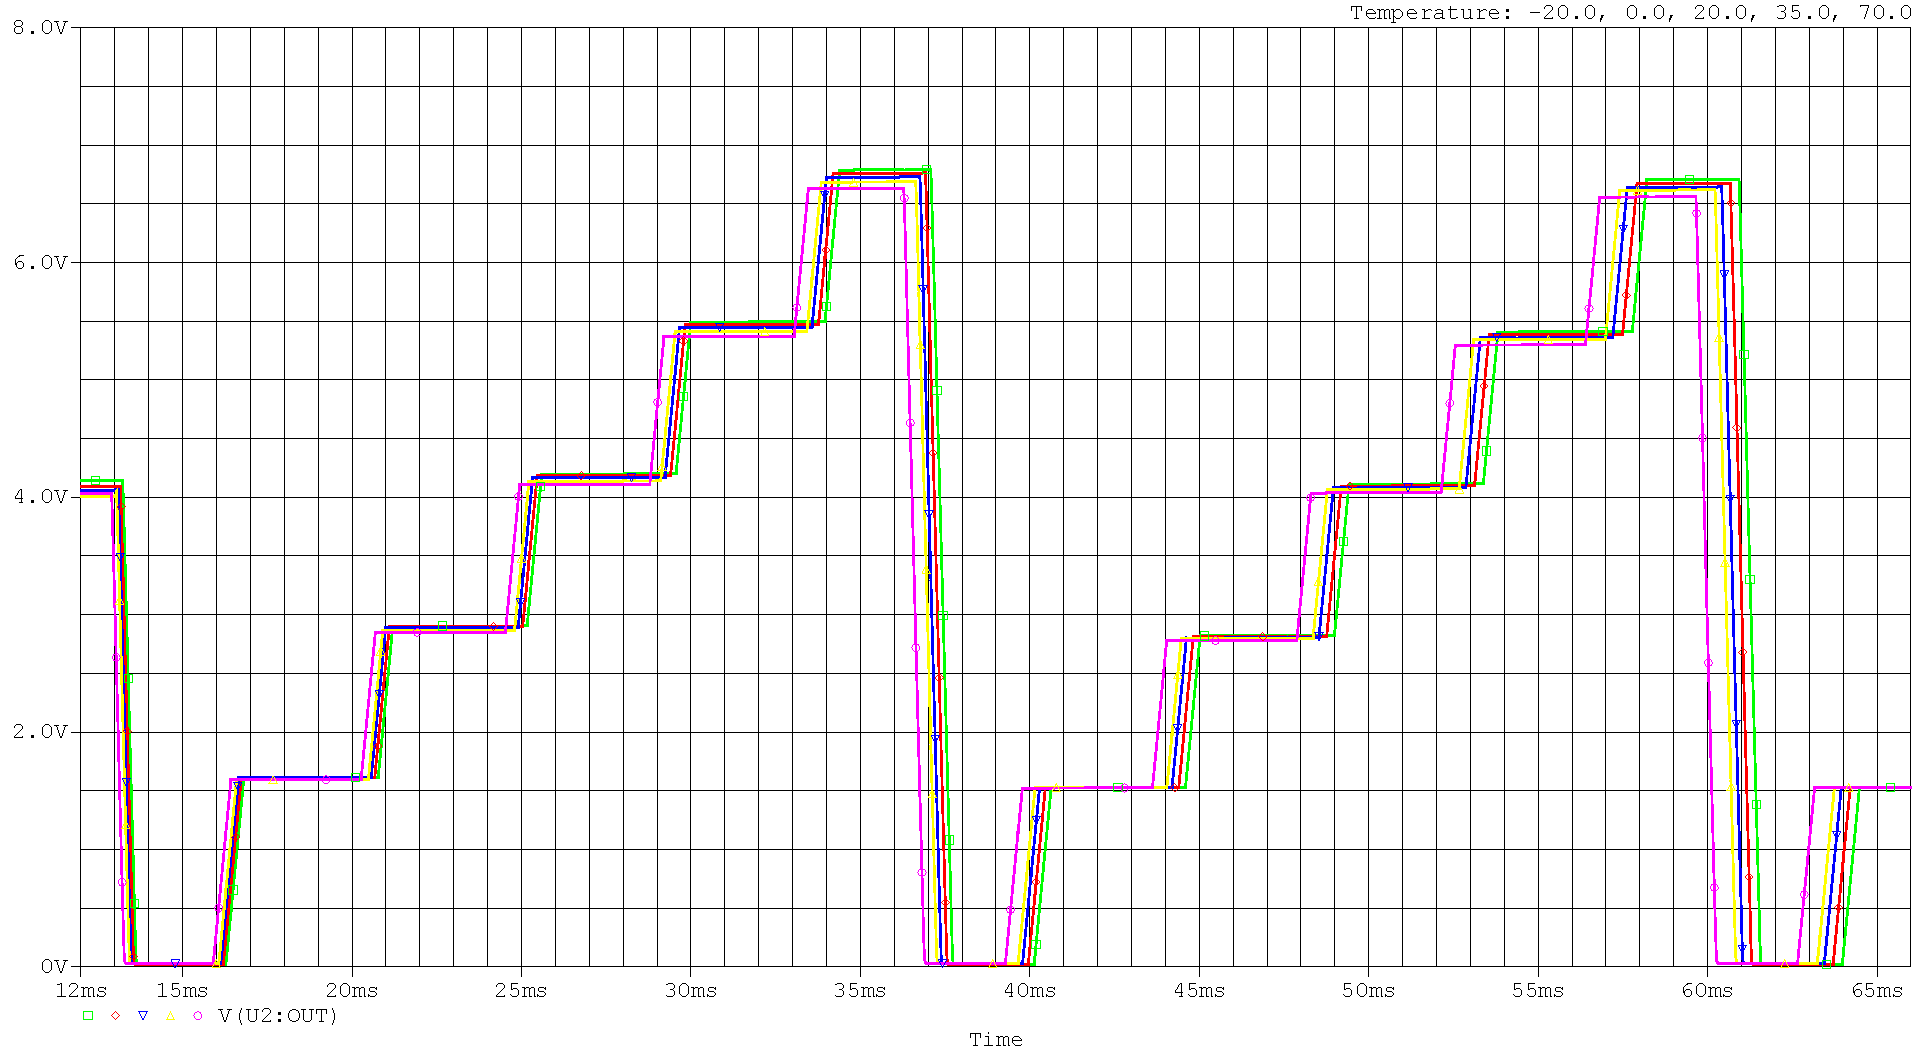
\includegraphics[width=13cm]{spice_02/q5.pdf}
	\label{plot:2_temp}
	\caption{Temperature sweep. Οι κυματομορφές στο υπόμνημα, από αριστερά προς δεξιά, αντιστοιχούν στις θερμοκρασίες $-20\unit{\celsius}$, $0\unit{\celsius}$, $20\unit{\celsius}$, $35\unit{\celsius}$ και $70\unit{\celsius}$.}
\end{plot_fig}
\vspace*{0.25cm}